\section{Dropping Policies} 
\label{sec:monitoring_dift_drop.policies}

In order to use partial monitoring to enable adjustable overhead, we must also
specify a policy for when and which monitoring events are dropped. In this
section, we discuss some of the options and trade-offs for dropping policies.
We split this decision into two components: 
\begin{enumerate} 
  \item When do we need to drop events in order to enable reduced overhead? (Section~\ref{sec:monitoring_dift_drop.policies.when}) 
  \item Which events should be dropped? (Section~\ref{sec:monitoring_dift_drop.policies.which}) 
\end{enumerate}

\subsection{Deciding When to Drop} 
\label{sec:monitoring_dift_drop.policies.when}

% Slack
\begin{figure} 
  \begin{center}
    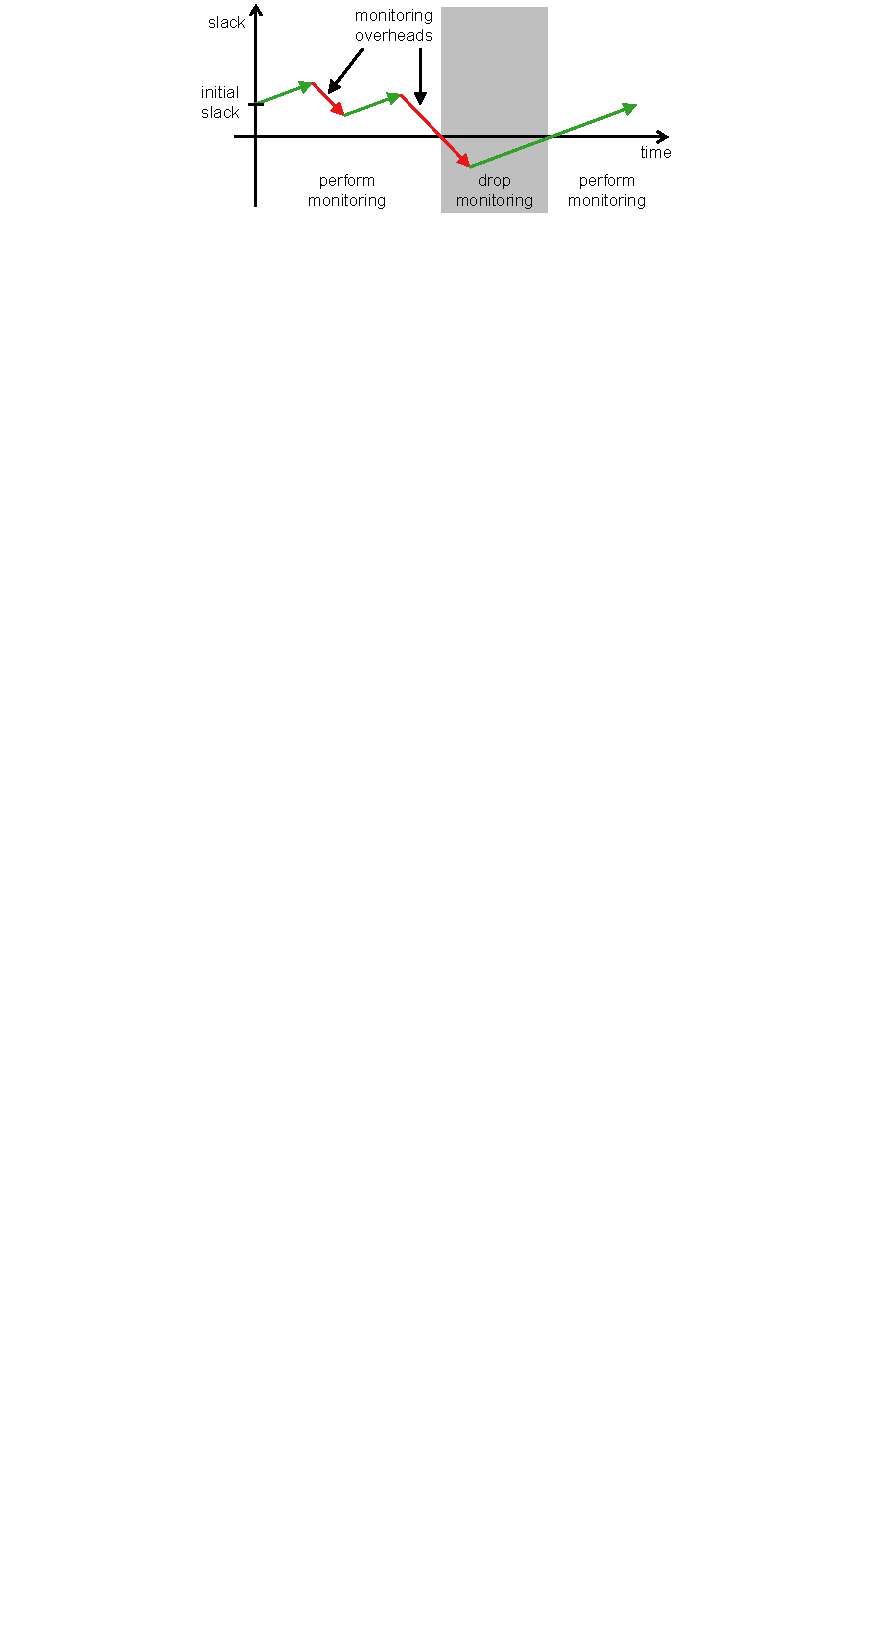
\includegraphics{monitoring_dift_drop/figs/slack.pdf} 
    \caption{Slack and its effect on monitoring over time.}
    \label{fig:monitoring_dift_drop.policies.slack} 
  \end{center} 
\end{figure}

In this section, we discuss two possible ways to determine when events should
be dropped.  The first possibility is to probabilistically drop events. By
setting the probability of dropping events appropriately, overhead can be
reduced. This works well for enabling partial monitoring for cooperative
testing and debugging since the randomness allows different users and runs to
monitor different portions of the program. However, using a probabilistic
dropping policy can make it difficult to meet a target overhead without prior
profiling.

Alternatively, we can specify a target overhead and estimate, at run-time, the
overhead of monitoring in order to decide whether dropping is needed.  The
overhead budget is specified as a percentage of the main program's execution
cycles without monitoring. In order to estimate the overhead at run-time, we
define \emph{slack} as the number of cycles of monitoring overhead that can be
incurred while staying within the budget target. Slack is essentially the
difference between the actual overhead seen and the budget specified. Note that
this definition differs slightly from the one used in
Chapter~\ref{chap:monitoring_hard_drop} where dynamic slack was the difference
between actual execution time and the worst-case execution time. Slack is
generated as the main program runs and consumed as monitoring overheads occur.
For example, if no monitoring overheads occur during 1000 cycles of the main
program's execution and the designer sets a 20\% overhead target, then the
slack that is built up during this period is 200 cycles. If the main core is
then stalled for 50 cycles due to monitoring, then the remaining slack is 150
cycles.  In addition to this accumulated slack, a small amount of initial slack
can be given in order for monitoring to be performed at the start of a program.
Figure~\ref{fig:monitoring_dift_drop.policies.slack} shows an example of how
slack can change over time.  In this slack-based policy, if the slack falls
below zero (i.e., the overhead budget is exceeded), then monitoring events are
dropped.

% Slack tracking module
\begin{figure} 
  \begin{center}
    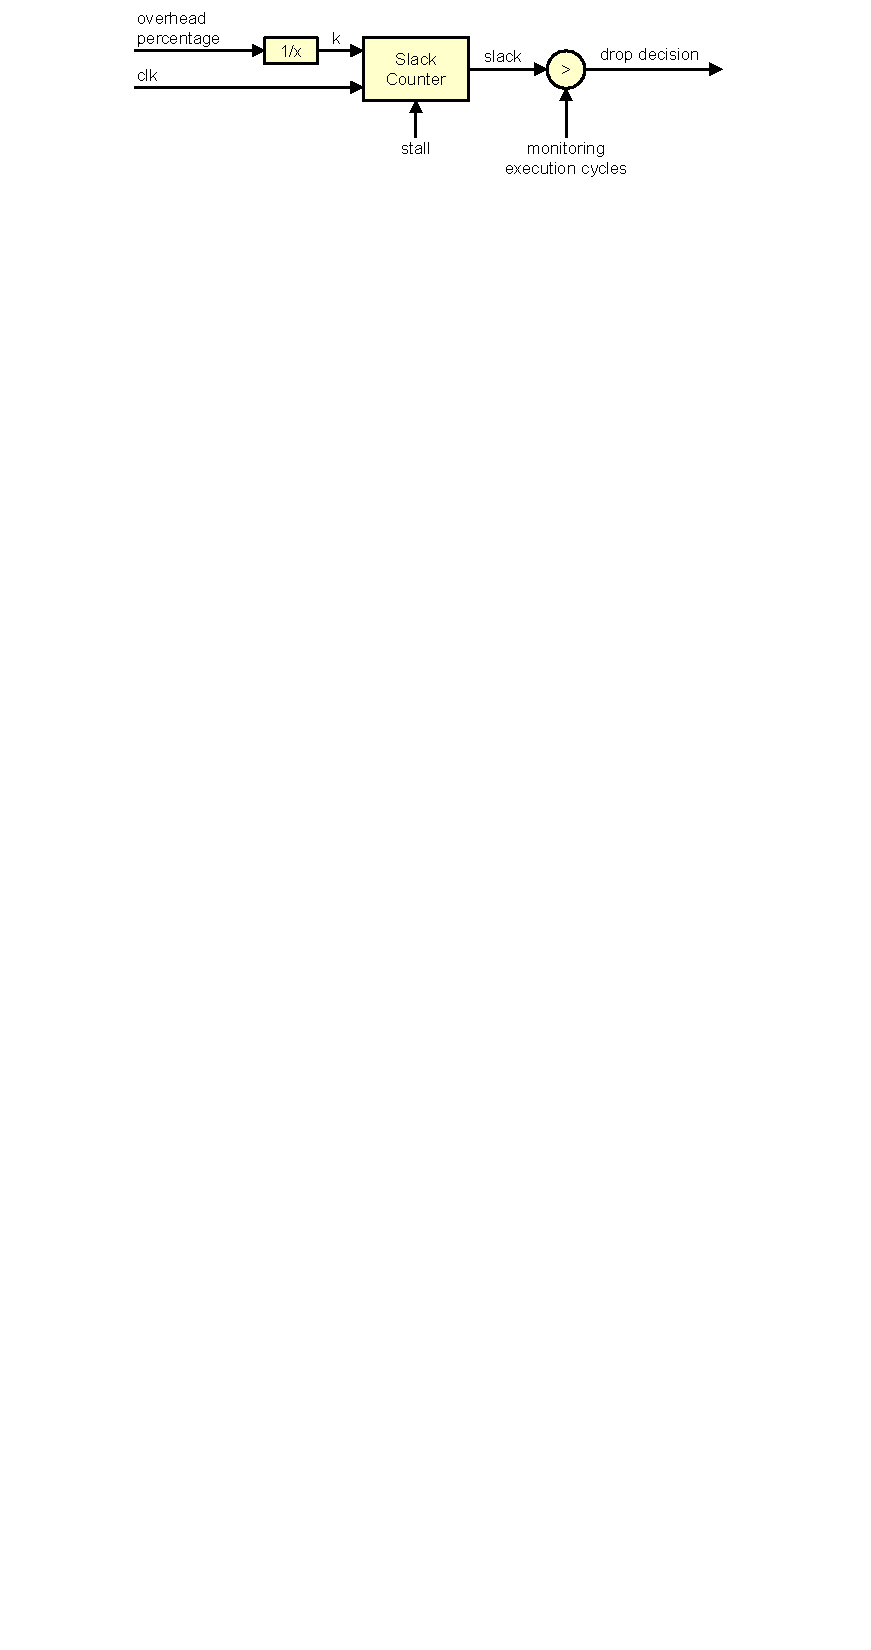
\includegraphics{monitoring_dift_drop/figs/slack_tracking.pdf} 
    \caption{Slack tracking and drop decision hardware.}
    \label{fig:monitoring_dift_drop.policies.slack_tracking} 
  \end{center} 
\end{figure}

Figure~\ref{fig:monitoring_dift_drop.policies.slack_tracking} shows how slack
can be easily measured in hardware by using a counter that increments on
every $k$-th cycle of the main core (e.g., every 5th cycle for a 20\% target
budget). The value of this counter is the accumulated slack. Whenever the main
core is stalled due to the monitor, the measured slack is decremented. It is
difficult to precisely determine the entire impact of monitoring on the main
core due to the difficulty in measuring certain overheads such as contention
for shared memory. However, we have found that using only the stalls due to
FIFO back pressure works well in practice.

\subsection{Deciding Which Events to Drop} 
\label{sec:monitoring_dift_drop.policies.which}

\begin{figure} 
  \begin{center} 
    \begin{subfigure}[Unrestricted Dropping] {
      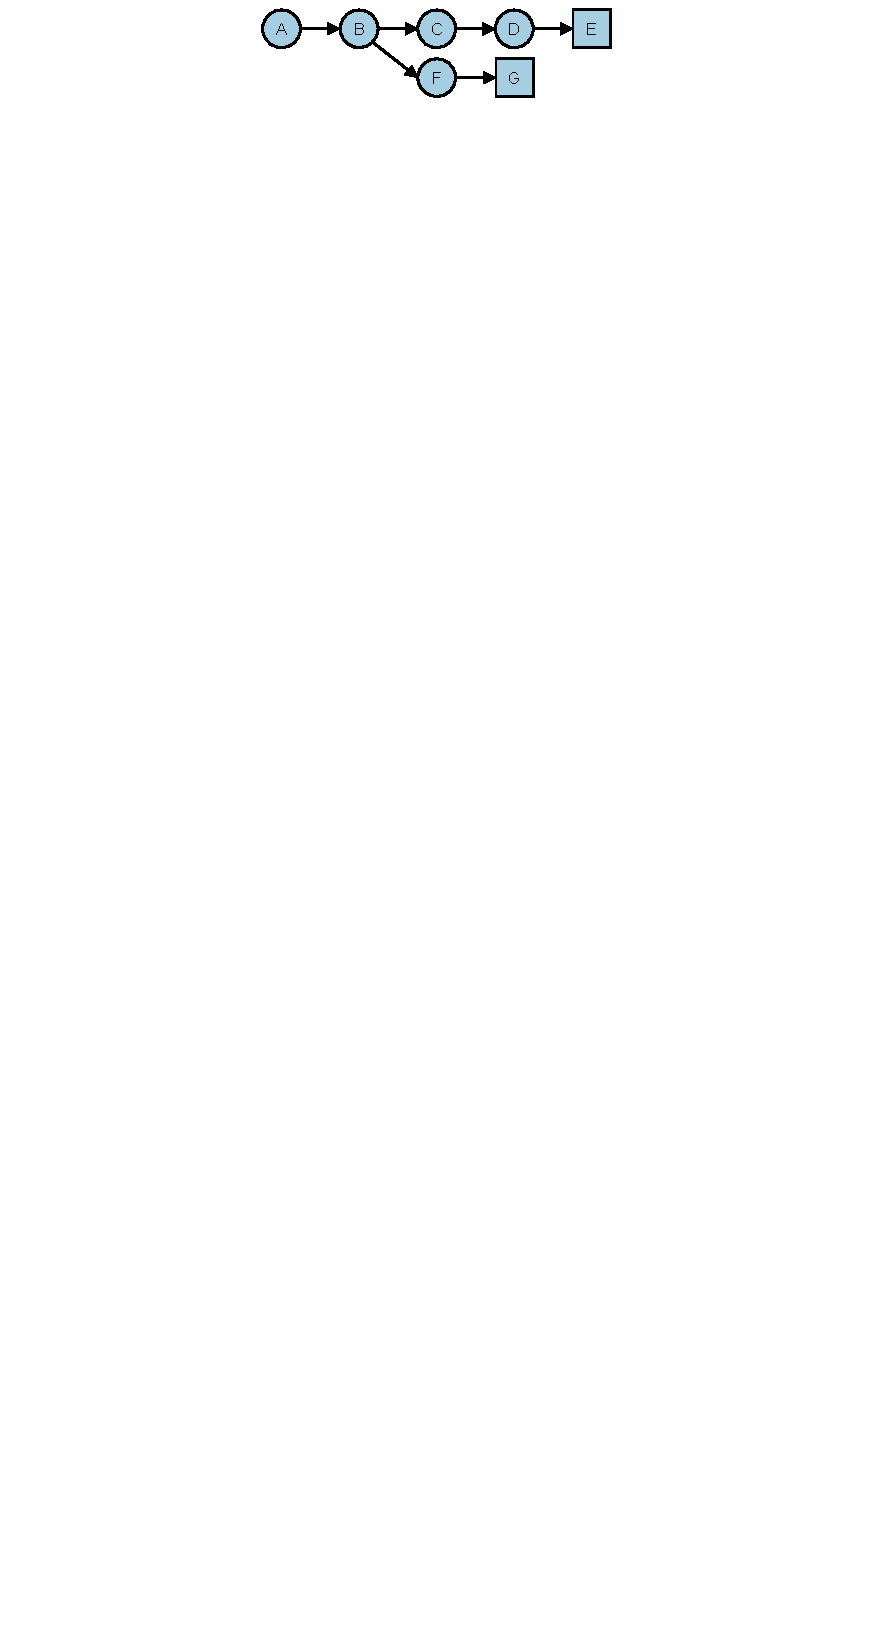
\includegraphics{monitoring_dift_drop/figs/unrestricted_drop.pdf}
      \label{fig:monitoring_dift_drop.policies.all_drop} 
    }
    \end{subfigure}
    \\
    \begin{subfigure}[Source-Only Dropping] { 
      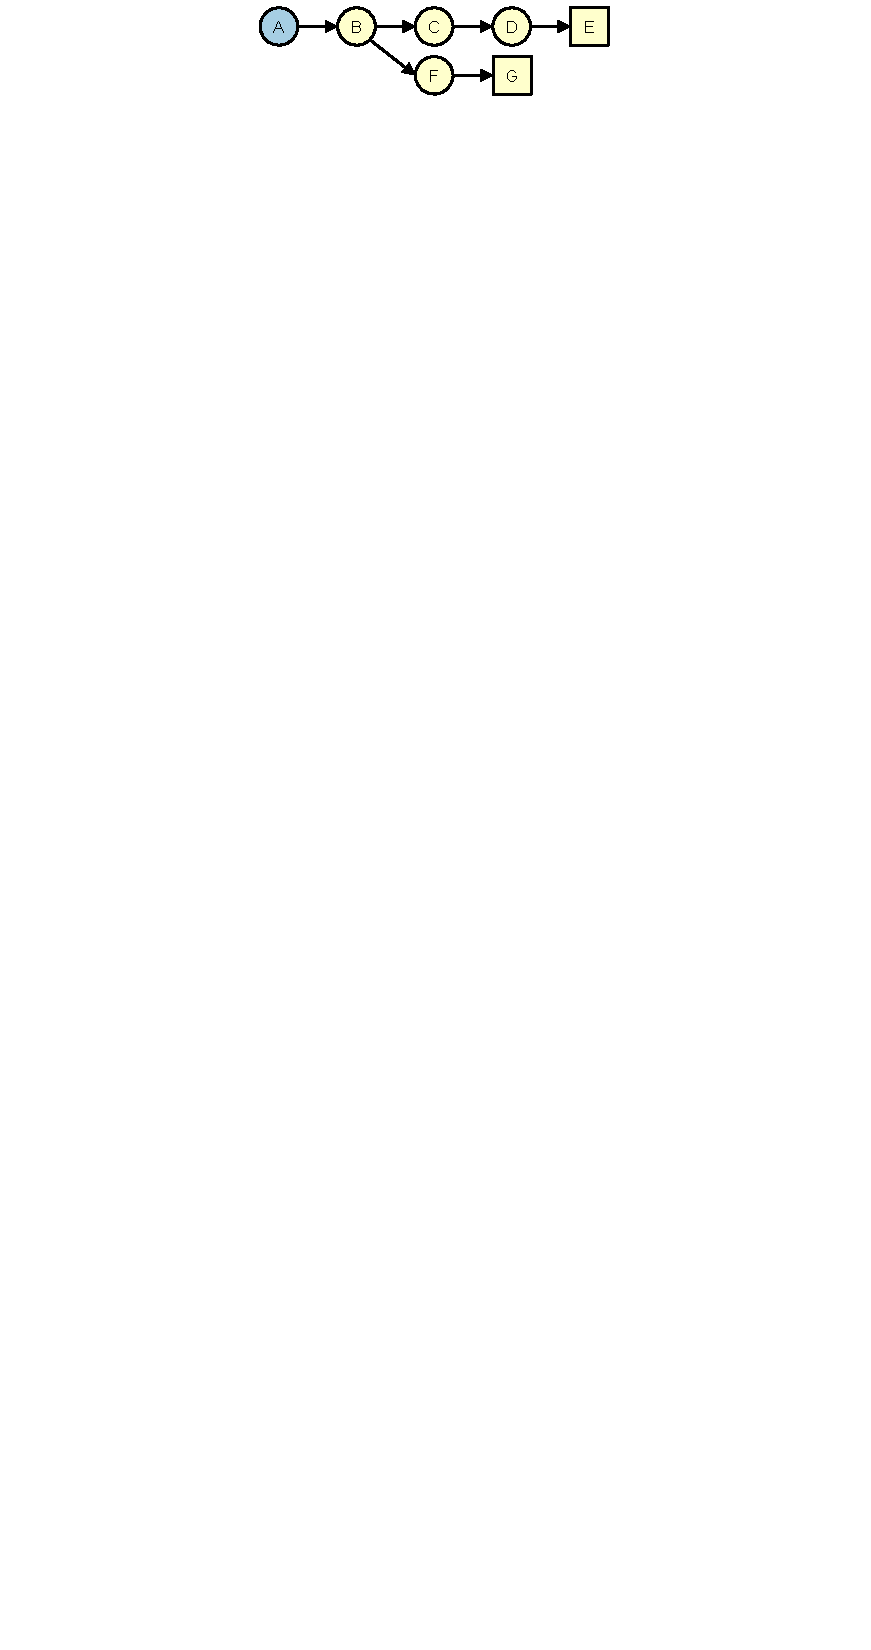
\includegraphics{monitoring_dift_drop/figs/source_drop.pdf}
      \label{fig:monitoring_dift_drop.policies.source_drop} 
    } 
    \end{subfigure}
    \\
    \begin{subfigure}[Sub-Flow Dropping] { 
      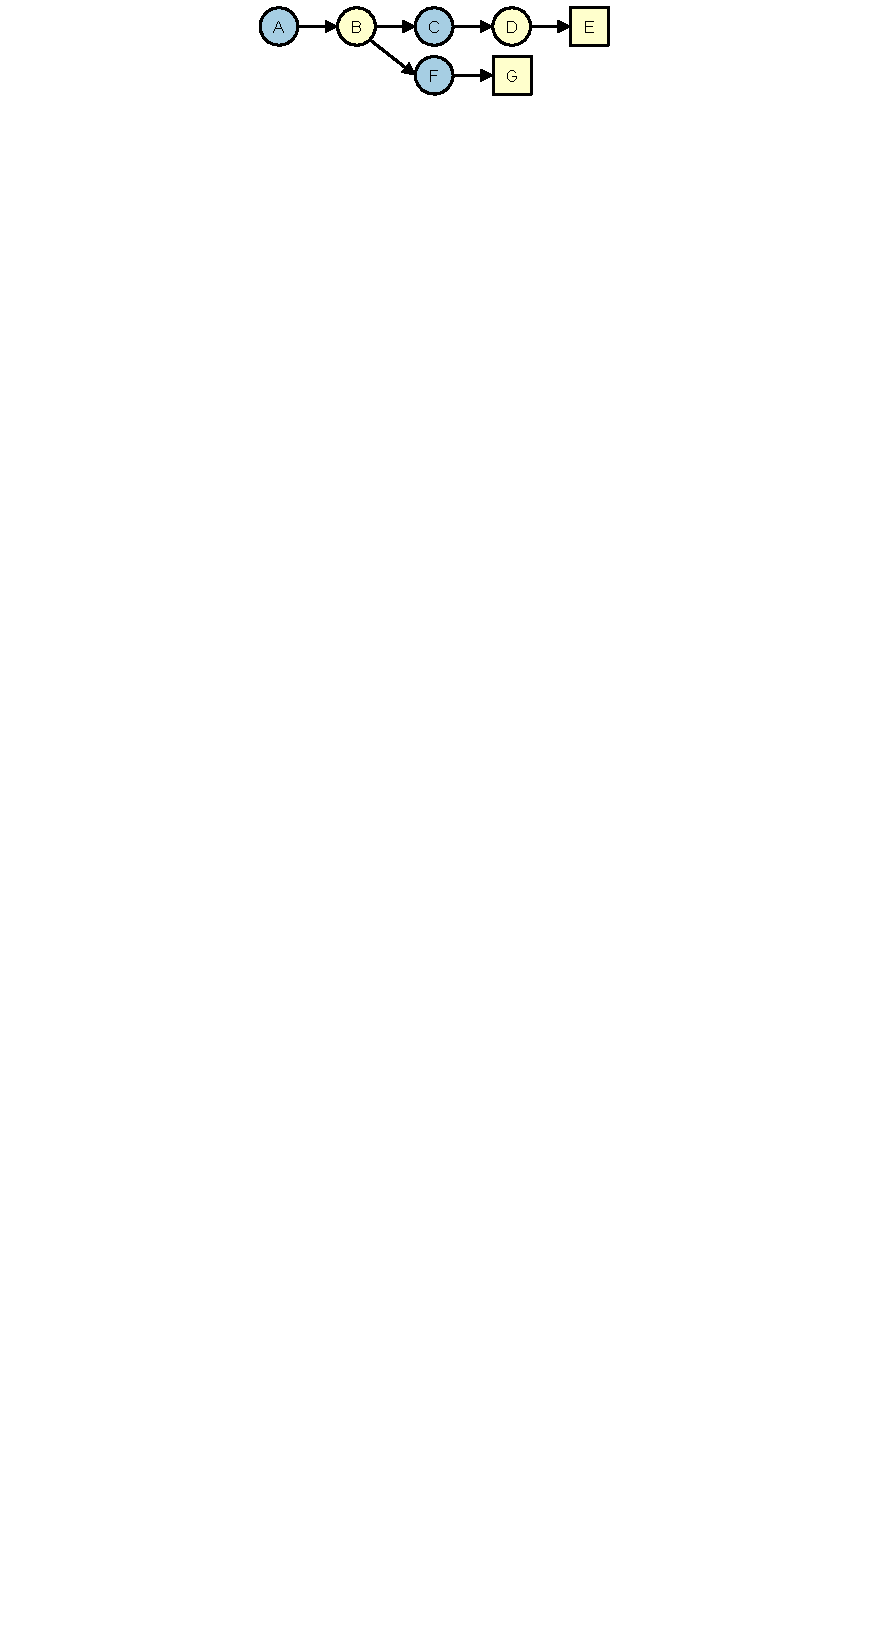
\includegraphics{monitoring_dift_drop/figs/subflow_drop.pdf}
      \label{fig:monitoring_dift_drop.policies.subflow_drop} 
    } 
    \end{subfigure}
  \end{center} 
  \caption{Comparison of dropping policies using metadata dependence graphs.
  Square nodes represent events where check are performed. Blue (dark) nodes
  indicate which nodes can be dropped.} 
  \label{fig:policies.policies} 
\end{figure}

In addition to deciding when dropping is required, trade-offs also exist in
deciding which events should be dropped.  The simplest policy is to drop
monitoring events when slack is less than or equal to zero.  However, this can
result in wasted work. For example, consider the metadata dependence graph
shown in Figure~\ref{fig:monitoring_dift_drop.policies.all_drop}. Here, an edge
from node {\tt A} to node {\tt B} represents that if event {\tt A} is dropped,
then due to its invalidated metadata, it will cause event {\tt B} to be
dropped. Square nodes indicate events where monitoring checks are performed. In
the example, suppose that event {\tt E} is meant to perform a check operation
but is dropped.  In this situation, the monitoring operations that were done
for events {\tt C} and {\tt D} were wasted since their results were not used
for any monitoring checks.  That is, by the time we decide to drop event {\tt
E}, we have already updated metadata for events {\tt C} and {\tt D} even though
they are no longer needed.

An alternative dropping policy which eliminates this wasted work is to only
make dropping decisions at the root or source of these metadata flows (see
Figure~\ref{fig:monitoring_dift_drop.policies.source_drop}). That is, we will
decide to either monitor or not monitor an entire metadata flow. An example of
these source nodes is the monitoring done to initialize base and bounds
information on {\tt malloc} for an array bounds check. These source nodes are
easily identifiable by the dropping hardware because they typically correspond
to the special instructions that are used to set up metadata information. Thus,
it is not necessary to generate and analyze the monitoring dependence graph to
identify source nodes. We refer to this dropping decision policy as
\emph{source-only dropping} and we refer to the previous policy of dropping any
event as \emph{unrestricted dropping}.

More complex dropping policies can be implemented given more detailed
information about the monitoring dependence graph. This information can be
found through static analysis or profiling, though we do not explore how to
find it in detail here. Given this information, we describe one possible policy
to use it, which we call \emph{sub-flow dropping}. Sub-flow dropping makes
dropping decisions at a granularity in between unrestricted dropping and
source-only dropping (see
Figure~\ref{fig:monitoring_dift_drop.policies.subflow_drop}).  The basic idea
of sub-flow dropping is to drop portions of the monitoring dependence graph at
the smallest granularity such that no work is wasted.  Sub-flow dropping allows
source nodes to be dropped and nodes after branch points in the monitoring
dependence graph to be dropped. From
Figure~\ref{fig:monitoring_dift_drop.policies.subflow_drop}, this corresponds
to nodes {\tt A}, {\tt C}, and {\tt F}. For example, dropping node {\tt C}
causes nodes {\tt D} and {\tt E} to be skipped. However, performing monitoring
on the remaining nodes allows the check at node {\tt G} to be performed with no
wasted work.  Similarly, dropping {\tt F} allows node {\tt E} to be checked
with no wasted work.  Note that sub-flow dropping can still result in wasted
work if there are merge points in the monitoring dependence graph and only part
of the incoming flows are dropped, but it should result in less wasted work
than compared to an unrestricted dropping policy. 

Source-only dropping will result in no wasted work and thus provide better
coverage than unrestricted dropping at a given overhead.  However, because of
the
coarser-grained decision, it may be more difficult to closely match overhead
targets.  Sub-flow dropping enables a design point in between unrestricted
dropping and source-only dropping in terms of matching overhead and coverage
achieved.  If the monitoring dependence graph is highly connected, then
source-only dropping will perform poorly. On the other hand, we expect
source-only dropping to work well when there are a large number of independent
metadata flows.  Monitoring dependence graphs with a large number of branches
will favor a sub-flow dropping policy.

The choice of dropping policy can also depend on whether probabilistic dropping
is performed instead of slack-based dropping.  Probabilistic dropping works
poorly with an unrestricted dropping policy. Since every event in a dependent
chain (e.g., events {\tt A} through {\tt E}) needs to be monitored in order for
the monitoring check to be useful, randomly dropping any event is likely to
cause the final check to be invalid by dropping at least one event in the
chain. Instead, source-only dropping works well when performing probabilistic
dropping.

Depending on the target application of partial monitoring, different policies
are more applicable.  For applications where closely matching an overhead
target is important, a slack-based, unrestricted dropping policy is
appropriate. However, if matching the overhead target is not as important, then
a slack-based, sub-flow or source-only dropping policy could provide better
coverage.  Finally, if the goal is to use partial monitoring to enable
cooperative debugging and testing with very low overhead, then a probabilistic,
source-only or sub-flow dropping policy can be used to provide good total
coverage over multiple runs.

